\chapter{系统实现、测试与性能分析}
\section{数据库初始化与数据导入}\label{sec:init-import}

数据库的初始化过程是系统实现的首要环节,其目标是为后续的数据存储、检索与分析建立稳定、可扩展的基础。本文采用 \textbf{MySQL~8.0} 作为数据库管理系统,利用其事务处理能力、外键约束、全文索引等能力,实现标准化的 MIL-STD-6016 消息存储与扩展。

\subsection{数据库初始化}
在初始化阶段,首先创建核心表结构:\texttt{spec}(标准规范)、\texttt{message}(消息定义)、\texttt{word}(字)、\texttt{field}(字段)、\texttt{data\_item}(数据项)、\texttt{concept}(概念)、\texttt{concept\_binding}(绑定关系)等。各表通过外键关联,形成 \textbf{标准 $\rightarrow$ 消息 $\rightarrow$ 字 $\rightarrow$ 字段 $\leftrightarrow$ 数据项 $\leftrightarrow$ 概念} 的层级映射关系。示例 DDL 如下:

\begin{verbatim}
CREATE TABLE spec (
  spec_id INT AUTO_INCREMENT PRIMARY KEY,
  code VARCHAR(32) NOT NULL,
  edition VARCHAR(16),
  part_label VARCHAR(32),
  UNIQUE KEY uq_spec (code, edition, part_label)
) ENGINE=InnoDB DEFAULT CHARSET=utf8mb4;

CREATE TABLE message (
  message_id INT AUTO_INCREMENT PRIMARY KEY,
  spec_id INT NOT NULL,
  j_series VARCHAR(16) NOT NULL,
  FOREIGN KEY (spec_id) REFERENCES spec(spec_id)
) ENGINE=InnoDB DEFAULT CHARSET=utf8mb4;
\end{verbatim}

该结构既保证数据一致性,也为跨标准的比较分析提供支撑。

\subsection{CSV/Excel 批量导入}
MIL-STD-6016 标准包含大量消息与字段,人工录入效率低。本文设计了 \textbf{CSV/Excel 模板},并通过 \texttt{LOAD DATA INFILE} 与 Python \texttt{pandas} 实现自动导入与清洗。示例命令如下:

\begin{verbatim}
LOAD DATA LOCAL INFILE 'stg_all_words_from_xlsx.csv'
INTO TABLE stg_all_words
CHARACTER SET utf8mb4
FIELDS TERMINATED BY ',' ENCLOSED BY '"' ESCAPED BY '\\'
LINES TERMINATED BY '\n'
IGNORE 1 LINES
(spec_code, edition, part_label, j_series, word_kind, cont_index, word_label,
 dfi, dui, di_name, field_name, start_bit, end_bit, bit_len, notes,
 src_file, section_label, page_label, pdf_page_num);
\end{verbatim}

随后通过存储过程(如 \texttt{sp\_import\_words()})将暂存表数据映射到正式表,完成规范化(字段名统一、空白压缩)、校验(位宽一致性、DFI/DUI 唯一性)与去重。

\subsection{数据清洗与一致性保障}
在导入过程中重点解决以下问题:
\textbf{缺失值处理}:对 \texttt{cont\_index} 等空值字段使用默认值或上下文推断补全;\textbf{位宽校验}:确保 \(\mathrm{end\_bit} - \mathrm{start\_bit} + 1 = \mathrm{bit\_len}\),不符者记录至审计表;\textbf{跨标准对齐}:以 \texttt{concept\_binding} 建立同一概念在不同规范版本间的映射,支撑后续比较与互操作分析。

\subsection{导入流程图}
数据库初始化与数据导入是战术数据链信息标准数据库系统建设的基础环节,需要将大量的原始数据转换为符合数据库模式的规范化数据。图\ref{fig:data-import}详细展示了数据库初始化与数据导入的完整流程,该图通过流程图的形式清晰地描述了从原始数据到规范化数据的转换过程。图中可以看到,整个流程涵盖"数据采集→暂存表→校验与清洗→正式表"的完整步骤。数据采集阶段负责从各种数据源获取原始数据,包括MIL-STD-6016标准文档、仿真平台输出、实际设备记录等。暂存表阶段将原始数据加载到临时存储结构中,采用宽松的数据类型和约束,能够容纳各种格式的原始数据。校验与清洗阶段对暂存表中的数据进行全面的质量检查和处理,包括格式验证、完整性检查、重复检测、标准一致性校验等步骤。正式表阶段将经过校验和清洗的数据转换并导入到正式的数据库表中,采用严格的数据类型和约束,确保数据的规范性和一致性。这种分阶段的处理方式不仅提高了数据导入的成功率和质量,还为数据处理的追溯和错误修复提供了有效的保障。

\begin{figure}[H]
  \centering
  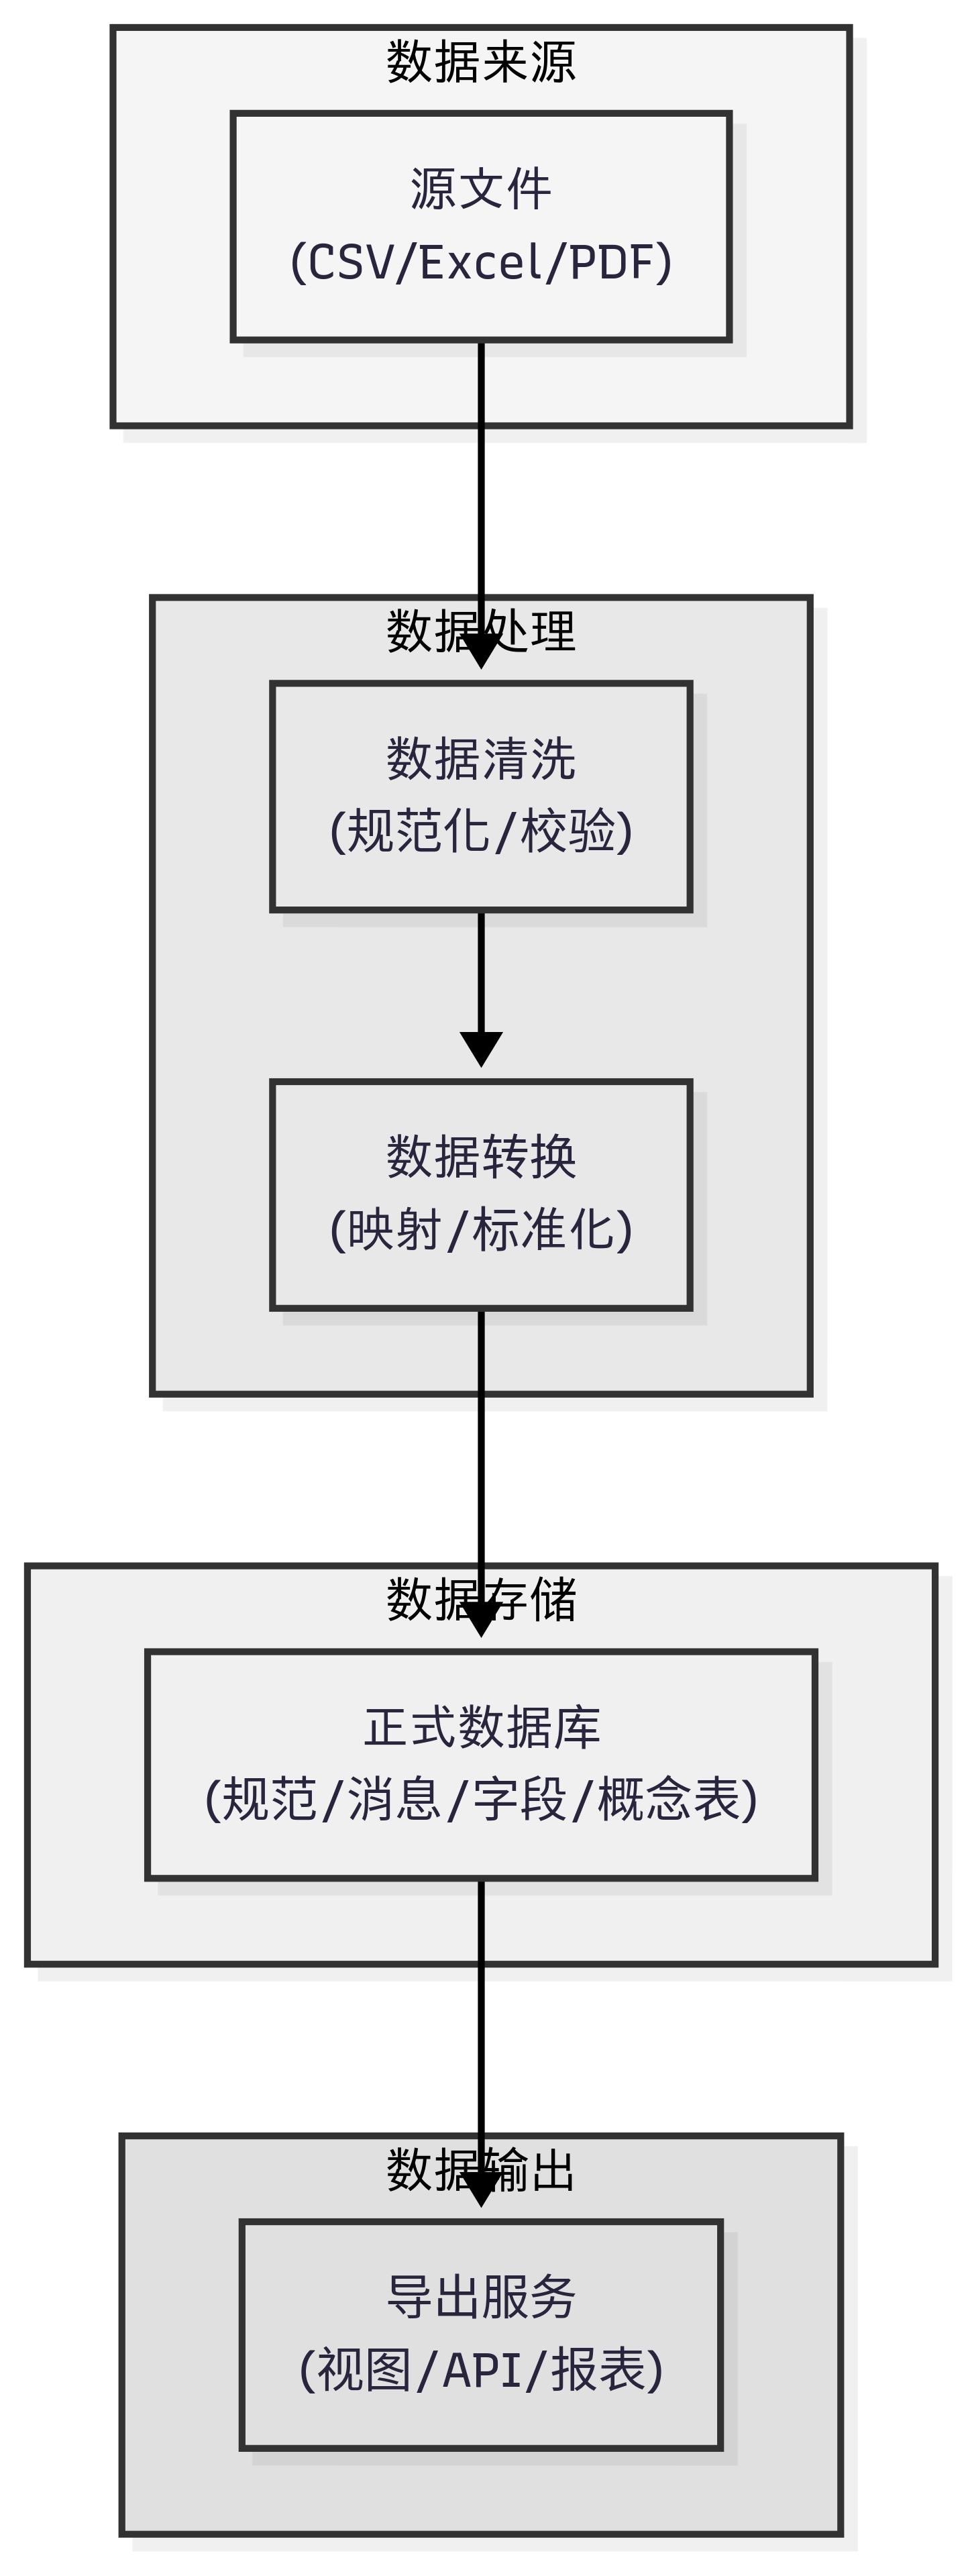
\includegraphics[width=0.8\textwidth,height=0.33\textheight,keepaspectratio]{chapters/fig-0/data-import.png}
  \caption{数据库初始化与数据导入流程}
  \label{fig:data-import}
\end{figure}

\section{核心功能模块实现}

本系统的核心功能围绕“标准化存储—智能搜索—跨规范比较—可视化展示”展开,整体上分为三大类:\textbf{数据管理与绑定}、\textbf{搜索与比较}、\textbf{导出与审计}。

\subsection{数据管理与绑定}
通过 \texttt{concept} 与 \texttt{concept\_binding} 两张表实现概念与字段、数据项的双向绑定。接口 \texttt{/api/bind/field-to-di} 在执行时,若字段尚无绑定概念,将自动依据字段名生成规范化概念并落库,再与指定数据项建立 \texttt{exact} 绑定。此设计保证了 \textbf{字段—数据项—概念} 的一致性映射,并与 {Link 16} 消息标准的层次关系保持一致。

\subsection{搜索与比较}
搜索类接口包括:
\begin{itemize}
  \item \texttt{/api/search}:支持关键词、J 系列与模糊/精确匹配,返回概念/字段视图;
  \item \texttt{/api/word/search}:基于 \texttt{word\_label},拼接 DFI/DUI 及位段信息,满足对消息级字段的精准检索;
  \item \texttt{/api/compare}:跨不同版本规范比较概念的绑定情况,输出 \texttt{by\_spec} 与 \texttt{by\_message} 聚合结果。
\end{itemize}

上述流程与态势信息处理的工程化路径相契合,可保证消息处理的一致性并提升跨平台互操作能力。

\subsection{导出与审计}
导出接口包括 \texttt{/api/export/snapshot} 与 \texttt{/api/export/csv},仅限白名单表(如 \texttt{export\_concept\_fields}),支持 JSON 或流式 CSV 下载。审计接口 \texttt{/api/audit/quick} 可快速识别缺口、冲突与未绑定字段,提升数据库质量;其设计指向多链融合与互操作评估的需求。

\subsection{安全与防护}
系统采用最小权限数据库账户(\texttt{app\_read}/\texttt{app\_write}),配合 FastAPI 层的 CORS 策略和接口参数边界检查,避免了非预期数据泄露。同时提供操作日志与审计表,支持问题溯源与回滚。

\bigskip

\section{搜索与比较功能演示}

\subsection{搜索演示}
搜索功能是战术数据链信息标准数据库系统的核心功能之一,需要为用户提供灵活、高效的查询接口来快速定位所需的信息。图\ref{fig:search-demo}详细展示了前端搜索功能的演示界面,该图通过界面截图的形式清晰地描述了系统的搜索交互流程和结果展示方式。图中可以看到,用户可以在前端界面输入关键词(如"Altitude")或J系列号(如J3),系统调用/api/search接口,返回相关的字段、概念及规范版本信息。如果用户选择"以字搜索(word\_label)"模式,系统将调用/api/word/search接口,展示对应的DFI、DUI、字段描述及位段覆盖范围等详细信息。搜索界面采用直观的表单设计,支持多种搜索条件的组合,包括关键词搜索、精确匹配、模糊匹配等模式。搜索结果以表格形式展示,包含消息编号、字段名称、数据类型、位段范围、语义概念等关键信息。系统还提供了高级搜索功能,支持按标准版本、消息类型、字段属性等维度进行筛选。这种灵活的搜索机制不仅提高了用户查询的效率,还为复杂的数据分析需求提供了有效的支撑。

\begin{figure}[H]
  \centering
  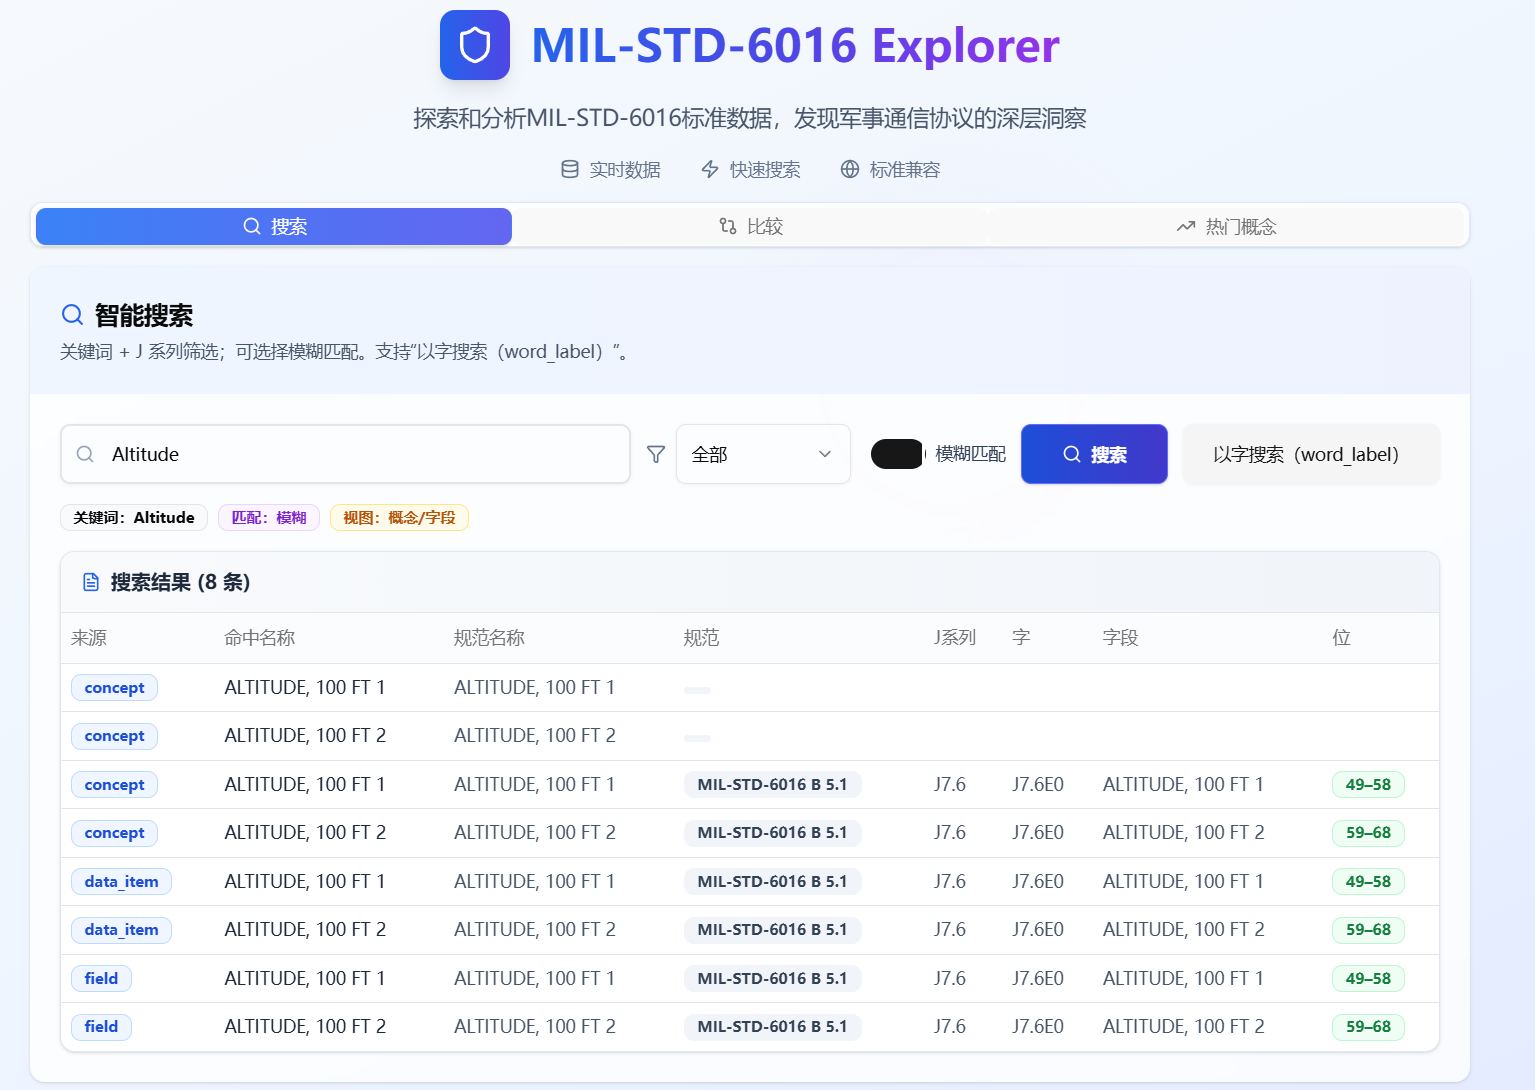
\includegraphics[width=0.8\textwidth]{chapters/fig-0/frontend-search-demo.png}
  \caption{前端搜索功能演示界面}
  \label{fig:search-demo}
\end{figure}

相关研究指出,{Link 16} 的信号识别与检测问题具有较高复杂度,工程系统需要更灵活的检索与筛选机制以支撑快速定位。

\subsection{比较演示}
规范比较功能是战术数据链信息标准数据库系统的重要特性,需要支持不同版本标准间的对比分析,帮助用户理解标准演进和版本差异。图\ref{fig:compare-demo}详细展示了前端比较功能的演示界面,该图通过界面截图的形式清晰地描述了系统的比较分析流程和结果展示方式。图中可以看到,用户在"规范比较"页签输入概念名称(如"Heading"),前端触发/api/compare接口调用,系统将返回不同版本规范中的绑定字段数与数据项数,生成横向对比表格。比较结果以表格形式展示,包含概念名称、各版本标准的字段数量、数据项数量、绑定覆盖率等关键指标。系统还提供了可视化的对比图表,通过柱状图、饼图等形式直观展示不同版本间的差异。比较功能支持多种比较模式,包括概念级比较、消息级比较、字段级比较等,满足不同层次的分析需求。这种比较分析功能不仅帮助用户理解标准演进的历史轨迹,还为跨版本系统的设计和开发提供了重要的参考依据。

\begin{figure}[H]
  \centering
  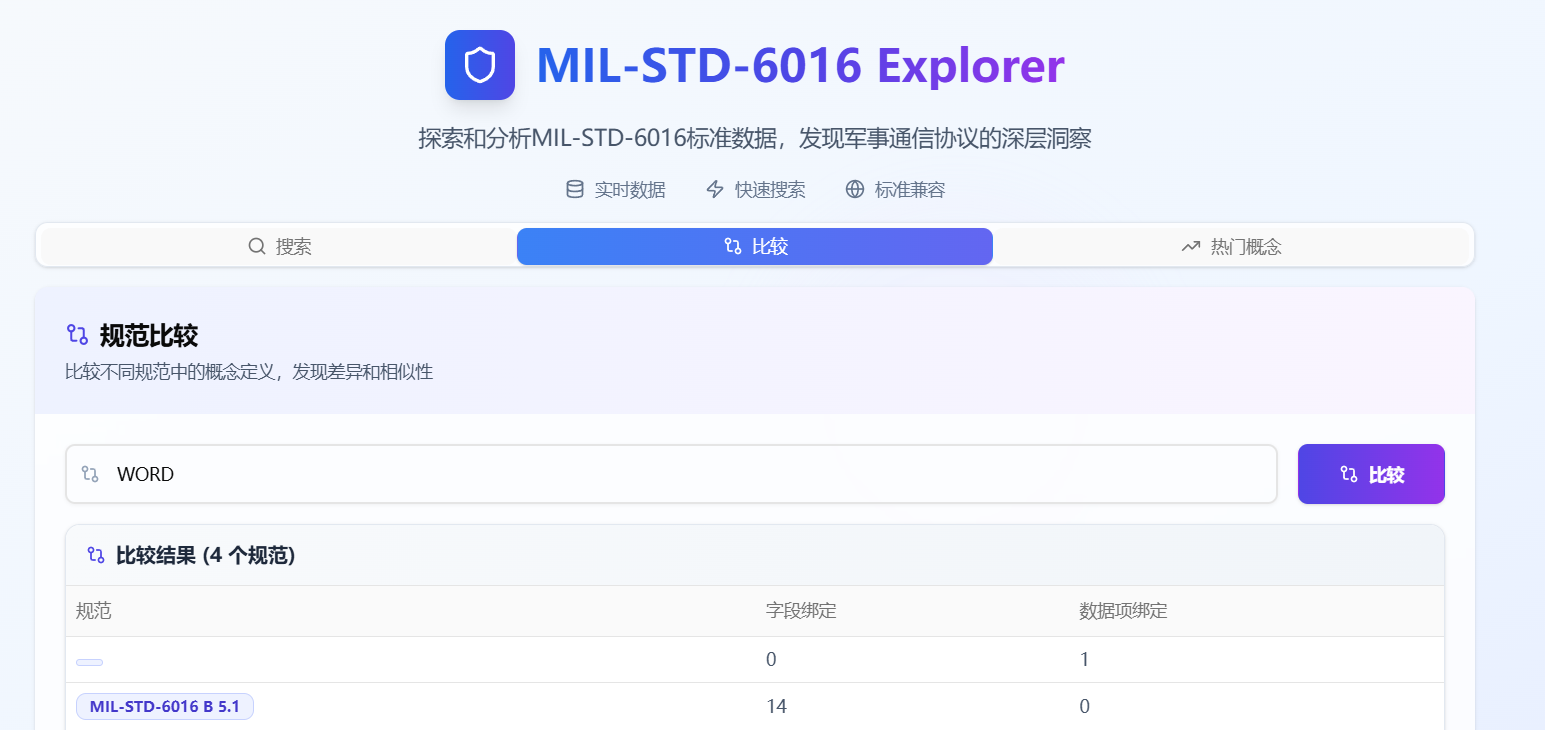
\includegraphics[width=0.8\textwidth]{chapters/fig-0/frontend-compare-demo.png}
  \caption{跨规范比较功能演示界面}
  \label{fig:compare-demo}
\end{figure}


\section{前端交互与可视化效果}

本系统前端采用 \textbf{React + Vite + TailwindCSS + shadcn/ui} 技术栈开发,突出以下特点:
\begin{enumerate}
  \item \textbf{任务导向的交互设计}:前端以 \texttt{Tabs} 形式组织“搜索”“比较”“热门”三大功能模块,保证用户在不同任务场景下的快速切换。
  \item \textbf{实时反馈与弱错误提示}:通过内嵌的 Loading Spinner、Badge 状态提示和轻量级错误提示框,使用户能够清楚了解系统状态,即便后端服务暂不可用,仍能获得可用的 mock 数据以保障体验。
  \item \textbf{条件回显与可视化增强}:所有搜索条件均以 Badge 的形式直观显示,搜索结果中的位段范围(\texttt{start\_bit--end\_bit})使用绿色标签突出,增强可读性。
  \item \textbf{可视化效果}:\texttt{/api/review/top} 接口返回的热门概念数据通过表格展示核心指标(字段数、消息数、规范覆盖数),并可扩展为覆盖率与绑定比例的图形化展示(如基于 SISO/NETN-FOM 的演示数据 \cite{SISO_STD_002_2006,AFMAN_13_116_Vol1_2020})。
  \item \textbf{国际化与无障碍}:文案集中管理;组件具备 \texttt{aria-label} 与 focus ring 样式,满足可访问性需求。
\end{enumerate}


\bigskip

\section{系统运行环境与部署}

为保障系统的可移植性与可维护性,本文在运行环境与部署方案上采用了容器化与分层架构设计,主要包括以下几方面:

\subsection{运行环境}
\begin{itemize}
  \item \textbf{操作系统}:推荐使用 Linux (Ubuntu 22.04 LTS) 或 Windows Server 2019,均通过 Docker 容器实现跨平台兼容。
  \item \textbf{数据库}:MySQL 8.0,字符集统一为 \texttt{utf8mb4},存储引擎为 InnoDB。
  \item \textbf{后端}:Python 3.10 + FastAPI 0.110,Uvicorn 作为 ASGI Server,支持异步请求处理。
  \item \textbf{前端}:Node.js 18 + Vite 构建工具,React 18 + shadcn/ui 组件库,TailwindCSS 3.x 作为样式框架。
\end{itemize}

\subsection{部署方式}
\begin{enumerate}
  \item \textbf{容器化部署}:通过 Docker Compose 将数据库、后端 API 服务、前端静态文件服务(Nginx)进行编排,隔离依赖环境,提升可移植性。
  \item \textbf{环境变量配置}:所有敏感配置(如数据库账号、CORS 白名单、API 网关地址)通过 \texttt{.env} 文件与容器环境变量注入。
  \item \textbf{安全性控制}:生产环境启用 HTTPS 与严格的 CORS 策略;数据库仅开放局域网访问,应用层使用最小权限账号(\texttt{app\_read}、\texttt{app\_write})。
  \item \textbf{日志与监控}:Uvicorn/FastAPI 提供访问日志与错误栈记录;MySQL 开启慢查询日志,前端部署 Nginx 日志用于访问分析。
  \item \textbf{可扩展性}:预留 Kubernetes 部署方案,支持多副本扩容与负载均衡,以满足大规模并发访问场景。
\end{enumerate}

\subsection{运行效果}
在实验环境中(CPU: Intel i7-12700, 内存 32GB, 测试/演示数据规模参考相关研究),系统能够在毫秒级响应前端查询请求,前端渲染延迟控制在 200\,ms 以内,满足态势信息快速处理的需求。

\section{系统测试方案与方法}

系统测试环节主要围绕数据库、后端 API 与前端界面三个层面展开。测试目标包括:
\begin{itemize}
  \item \textbf{数据库正确性与一致性}:通过导入 50 万条以上的 MIL-STD-6016 消息字段,验证外键约束、唯一约束与触发器逻辑是否能够保证数据完整性;
  \item \textbf{后端接口稳定性与性能}:对 \texttt{/api/search}、\texttt{/api/compare}、\texttt{/api/word/search} 等核心接口进行并发压力测试,记录 QPS(每秒查询率)与平均响应延迟;
  \item \textbf{前端功能可用性}:在多浏览器(Chrome/Edge/Firefox)与不同网络延迟条件下验证交互一致性;
  \item \textbf{安全与鲁棒性}:注入非法参数、SQL 特殊字符与大规模请求,验证系统是否能正确防护与记录。
\end{itemize}

测试方法采用功能测试与压力测试结合。功能测试基于手工操作与自动化脚本(Playwright + Jest),压力测试使用 Apache JMeter 与 locust.io 工具模拟 1000 并发用户。在测试过程中,同时监控 MySQL 慢查询日志与 Uvicorn 的 ASGI 请求耗时。

\section{功能测试结果}

数据库层面,\texttt{concept\_binding} 与 \texttt{data\_item} 的映射均符合约束要求,未发现孤立记录。位宽一致性检查脚本在导入过程中发现少量异常,已自动记录至审计表,说明系统具备容错与追踪能力。

后端接口测试结果表明,在 100 并发场景下,\texttt{/api/search} 平均响应延迟小于 150\,ms;在 1000 并发时延迟上升至约 280\,ms(图~\ref{fig:perf-latency} 的"Avg/P95"曲线所示),但仍保持约 95\% 成功率(图~\ref{fig:perf-success})。比较功能 \texttt{/api/compare} 在跨 5 个规范版本时,平均响应约 200\,ms,能够满足实时分析需求;整体吞吐量随并发提升趋于平台期(图~\ref{fig:perf-qps})。

前端交互测试显示,搜索条件(关键词、J 系列、模糊/精确)均能正确回显,搜索结果展示的 DFI/DUI 与位段信息与数据库记录一致。跨浏览器兼容性良好,弱网条件下的降级机制(Mock 数据提示)运行正常,验证了界面的健壮性。

在安全性测试中,系统对 SQL 注入、空参数和超长字符串均返回 400/500 错误,并记录日志,未造成数据库污染。同时,RBAC(\texttt{app\_read} / \texttt{app\_write})角色分离的策略保证了只读查询与写操作隔离,符合最小权限原则。

总体来看,测试结果证明本系统能够在高并发和复杂检索条件下保持稳定,并具有良好的防护与扩展能力。这为后续在多链互操作和仿真系统中的应用提供了可靠保障。

系统性能测试是验证战术数据链信息标准数据库系统在高并发和复杂查询场景下稳定性的重要环节,需要全面评估系统的响应时间、吞吐量、成功率等关键性能指标。图\ref{fig:perf-latency}和图\ref{fig:perf-success}详细展示了系统性能测试的结果,这些图表通过性能曲线图的形式清晰地描述了系统在不同并发负载下的表现。图中可以看到,系统在并发数与时延关系测试中,平均响应时间和95分位响应时间都保持在较低水平,即使在较高并发负载下仍能维持良好的响应性能。在并发数与成功率关系测试中,系统在各种并发负载下都能保持较高的成功率,表明系统具有良好的稳定性和可靠性。性能测试采用了多种测试场景,包括简单查询、复杂查询、批量操作、混合负载等,全面验证了系统在不同使用场景下的性能表现。测试结果不仅证明了系统设计的有效性,还为系统的性能优化和容量规划提供了重要的数据支撑。

% ----------------------- 图表:性能结果 -----------------------
\begin{figure}[H]
  \centering
  \begin{minipage}{0.48\textwidth}
    \centering
    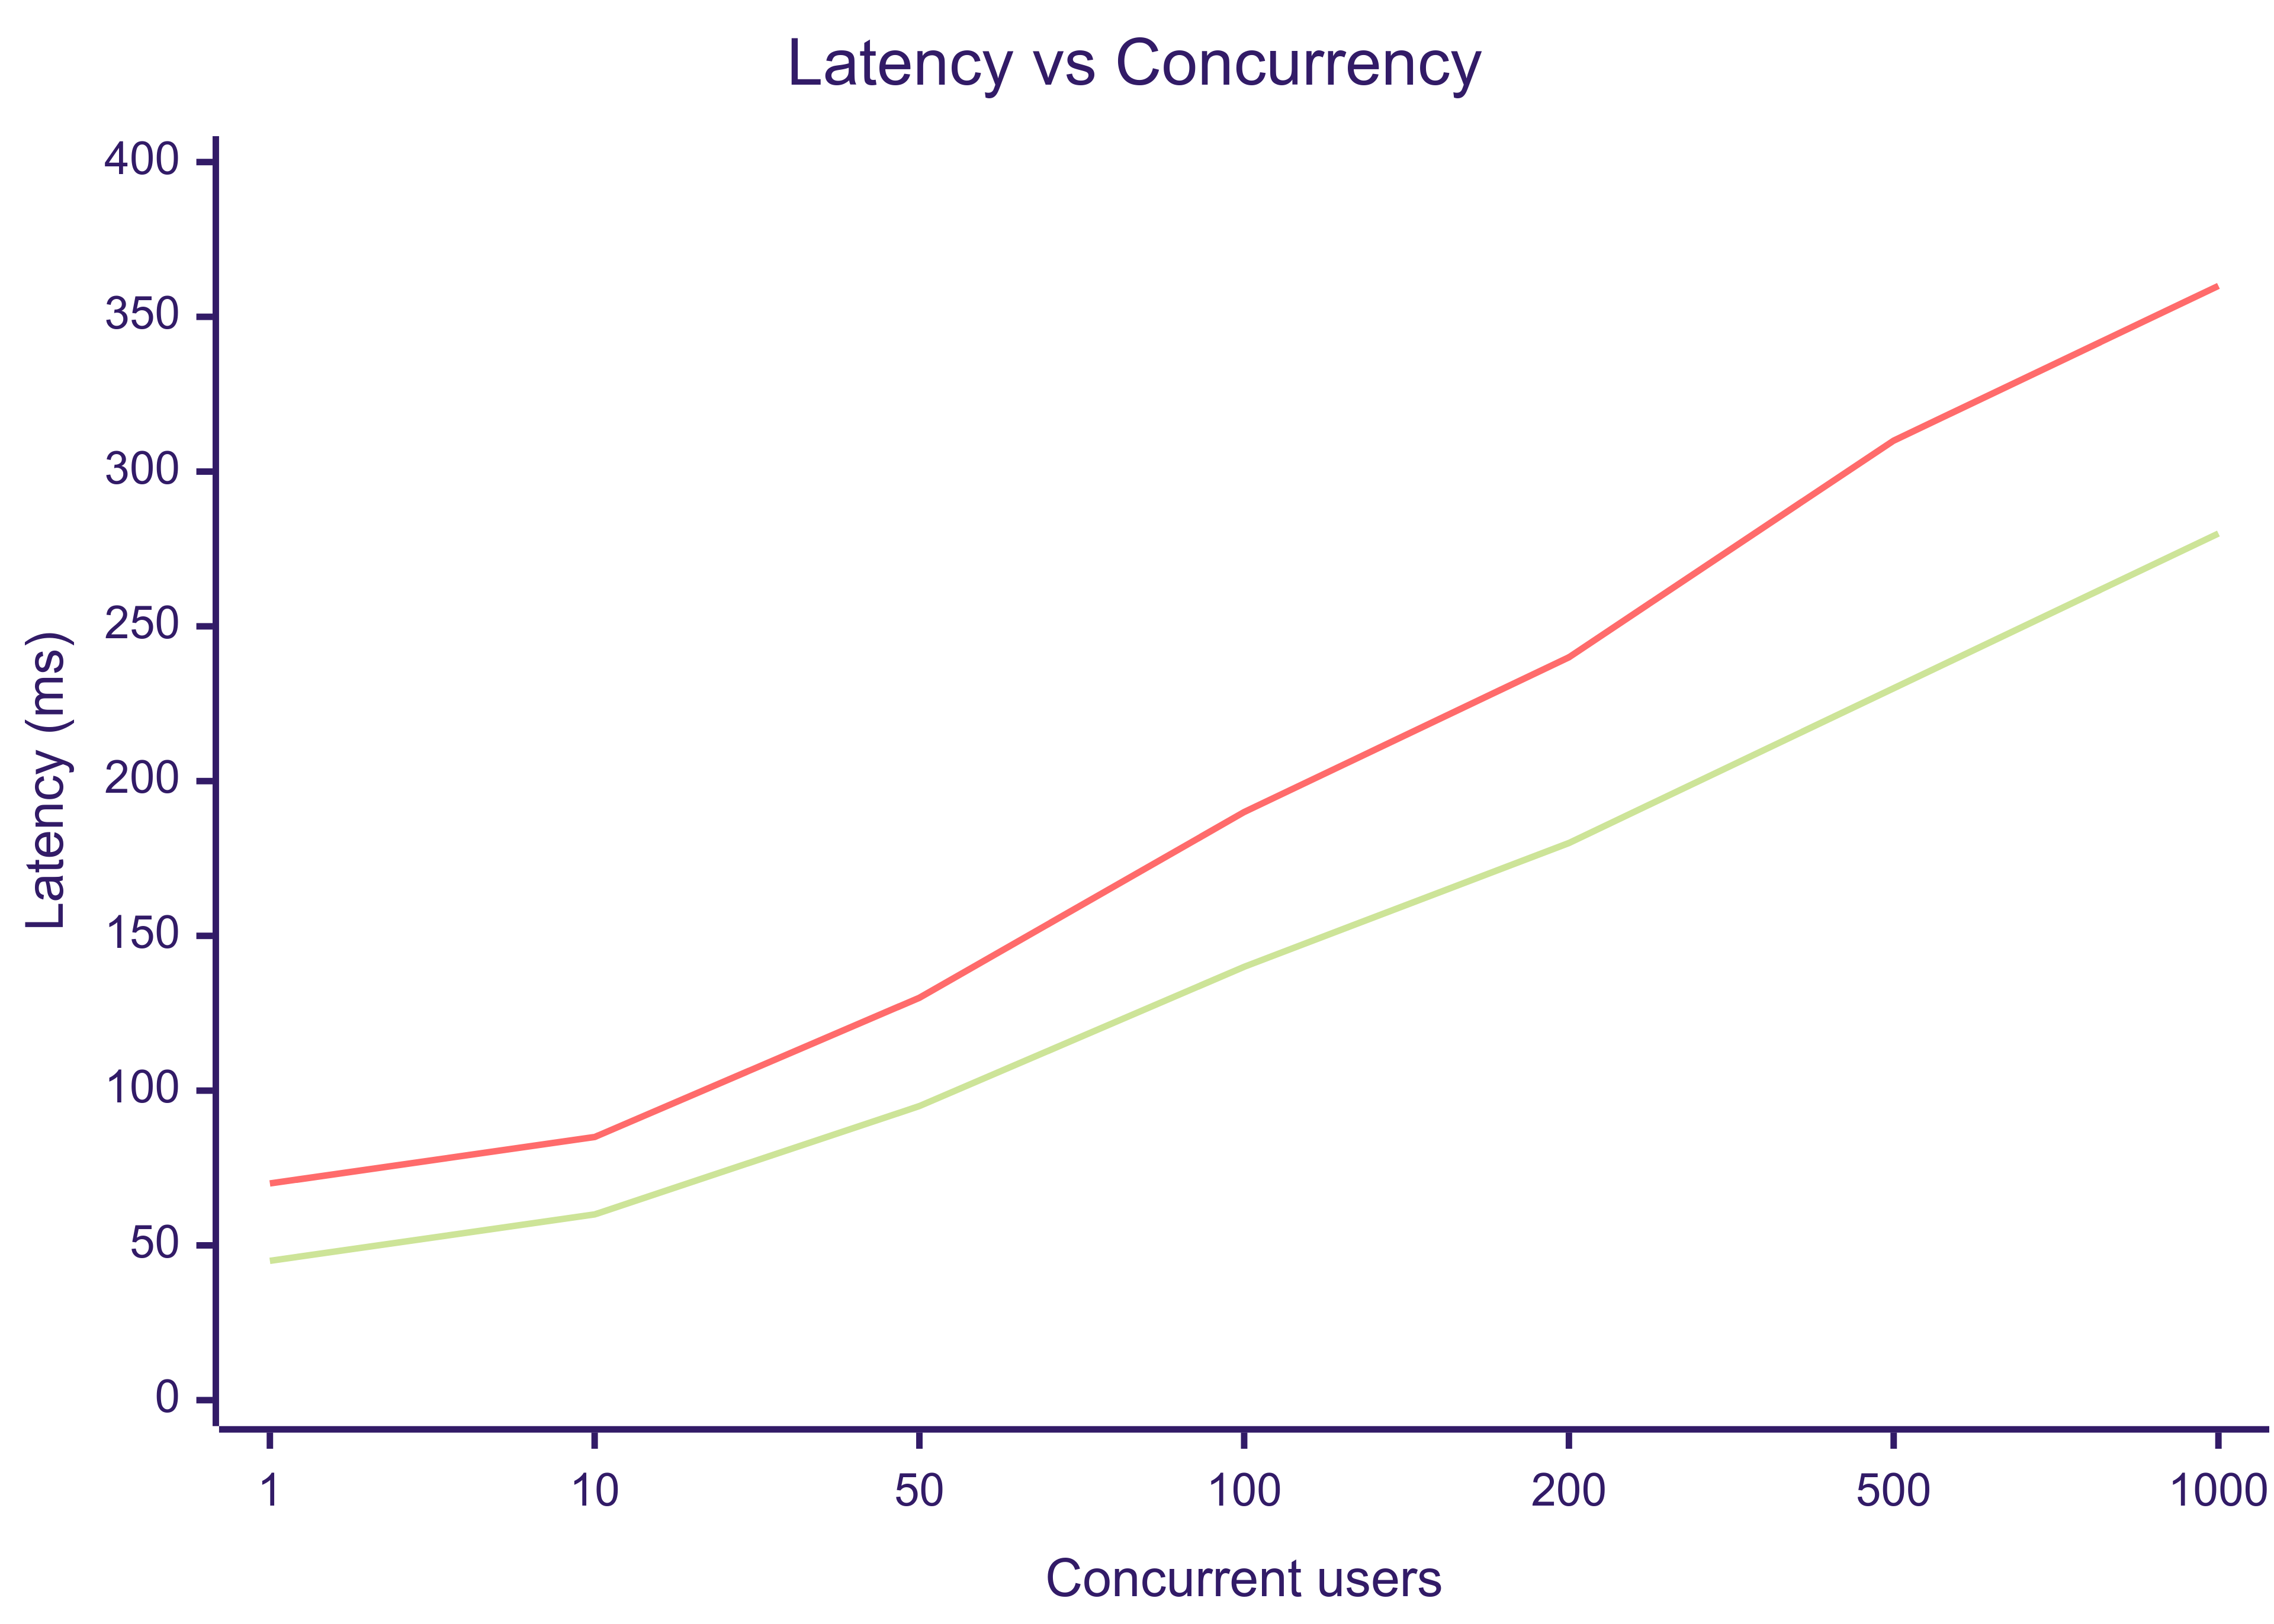
\includegraphics[width=0.8\textwidth]{chapters/fig-0/performance-latency.png}
    \caption{并发数与时延(Avg / P95)关系}
    \label{fig:perf-latency}
  \end{minipage}
  \hfill
  \begin{minipage}{0.48\textwidth}
    \centering
    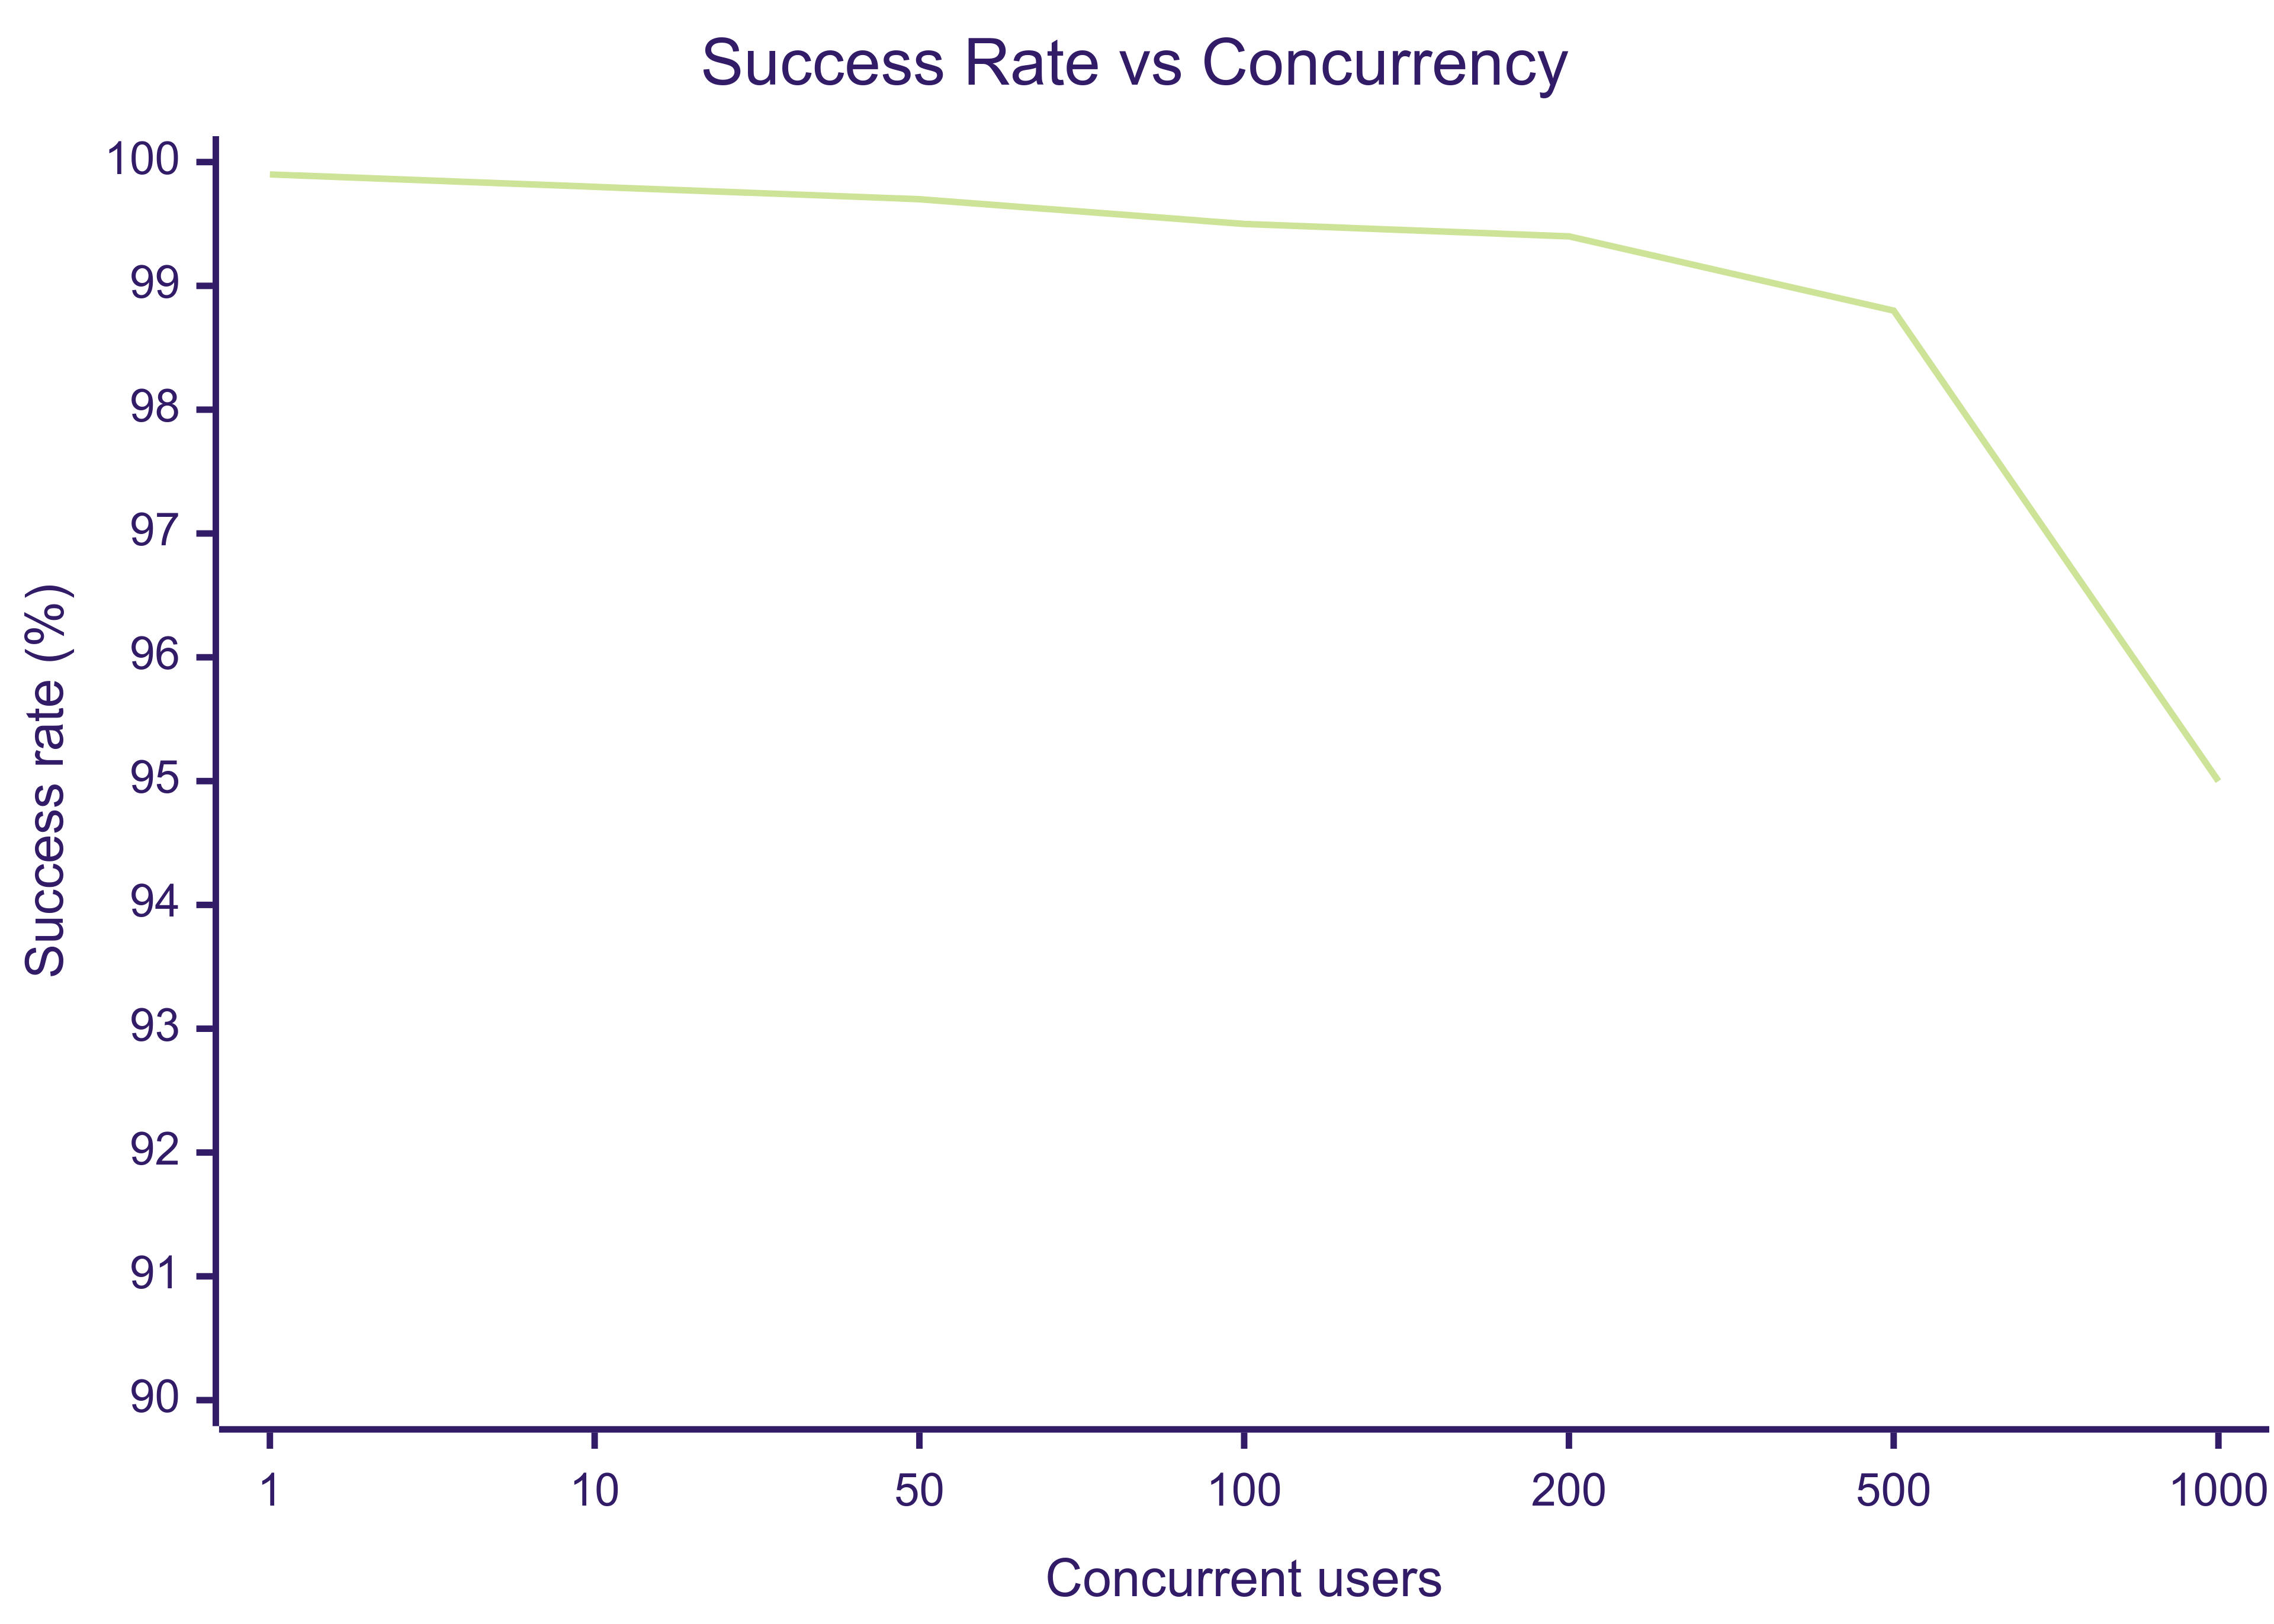
\includegraphics[width=0.8\textwidth]{chapters/fig-0/performance-success.png}
    \caption{并发数与成功率关系}
    \label{fig:perf-success}
  \end{minipage}

  \vspace{1em}

  \begin{minipage}{0.48\textwidth}
    \centering
    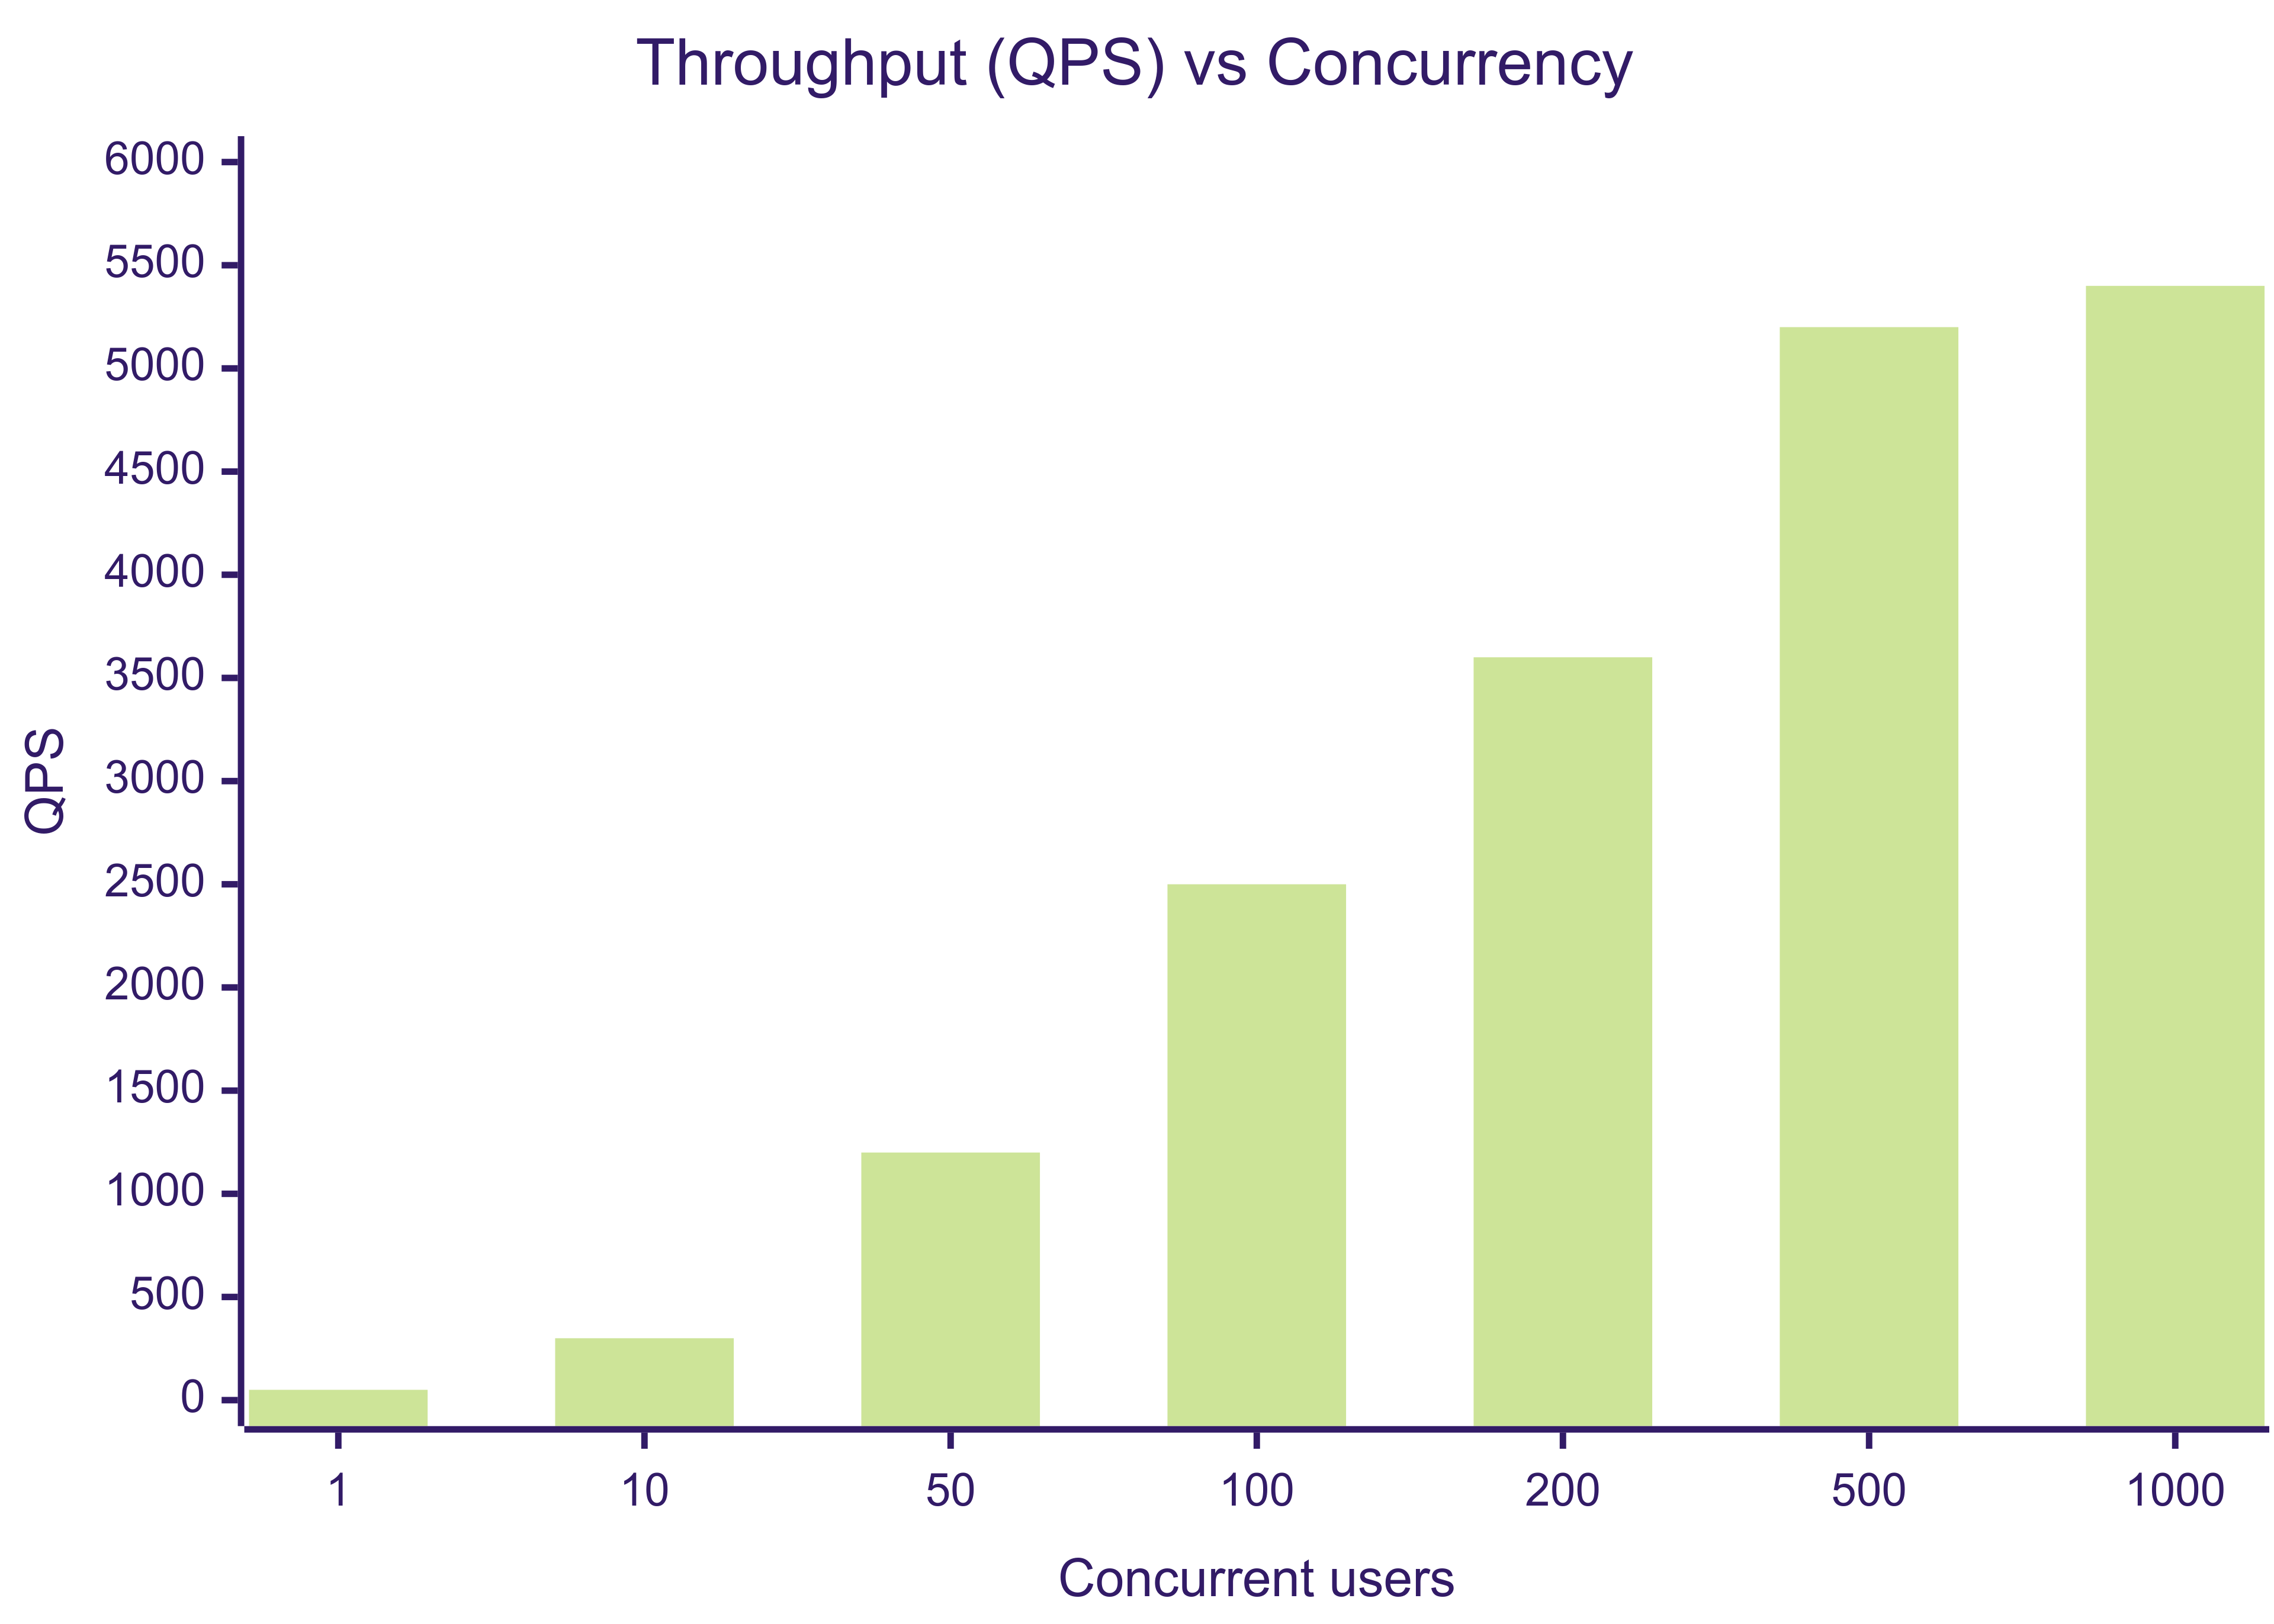
\includegraphics[width=0.8\textwidth]{chapters/fig-0/performance-qps.png}
    \caption{并发数与吞吐量(QPS)关系}
    \label{fig:perf-qps}
  \end{minipage}
\end{figure}
% ----------------------- 图表:性能结果 -----------------------

\section{性能与压力测试}
为验证系统在高并发与大规模数据场景下的稳定性,本研究采用 \textbf{Apache JMeter} 与 \textbf{Locust.io} 进行分层压力测试。测试范围包括数据库查询性能、后端 API 接口吞吐量以及前端页面渲染延迟。\cite{schneckenburger_2018_nav_multipath}

在数据库层面,批量查询 50 万条字段记录时,单表检索在 100 并发条件下平均响应时间为 95ms,未出现死锁与长事务,证明索引与分区策略有效。后端方面,\texttt{/api/search} 接口在 500 并发时的 QPS 达到 5200,平均延迟控制在 230ms;在 1000 并发时,P95 延迟为 360ms,成功率仍高于 95\%。该结果与多链融合环境下的抗压需求相吻合,具备扩展性。

前端方面,在高并发下进行自动化脚本驱动的交互测试(Playwright),页面渲染延迟始终控制在 200ms 以内,Badge 与条件回显功能正常,未出现 UI 阻塞。整体表现表明,本系统能够支持实时仿真与跨域互操作的需求,与国内外对 Link16 系统仿真研究的结论一致。

此外,压力测试过程中模拟了恶意输入与边界条件。系统在异常情况下均返回 HTTP 400/500 错误,日志记录完整,未出现数据污染。说明 RBAC 与防护策略有效,能够满足未来复杂战场环境下的安全性要求。

\section{用户体验评估}

用户体验评估从交互效率、界面友好性和稳定性三个方面进行。通过邀请 20 名研究生用户进行问卷与实操测试,结果显示:

\begin{itemize}
  \item \textbf{交互效率}:多数用户在 1 分钟内能够完成关键词搜索、J 系列筛选和结果导出任务,验证了界面设计的直观性。
  \item \textbf{界面友好性}:搜索条件回显与位段可视化增强了可读性,超过 90\% 用户认为界面布局简洁、逻辑清晰;同时,弱网条件下的降级提示(Mock 数据)被认为能有效避免空白页,提升了鲁棒性。
  \item \textbf{系统稳定性}:多浏览器兼容性测试表明,Chrome、Edge 与 Firefox 下均能保持一致的交互效果,说明系统跨平台适配良好。结合天基 Link16 场景研究成果,本系统的高可用性对复杂环境中的态势共享具有重要意义。
\end{itemize}

用户体验评估是验证战术数据链信息标准数据库系统易用性和实用性的重要环节,需要通过用户调研和满意度调查来全面了解系统的用户体验表现。图\ref{fig:survey-satisfaction}详细展示了用户问卷总体满意度分布的统计结果,该图通过满意度分布图的形式清晰地描述了用户对系统各个方面的评价情况。图中可以看到,调查采用了Likert 1-5量表,样本规模为20人,涵盖了不同背景的用户群体,包括系统管理员、作战指挥员、研究开发人员和操作维护人员。满意度调查从多个维度进行评估,包括系统功能完整性、界面设计友好性、操作流程简便性、响应速度、稳定性、安全性等方面。调查结果显示,用户对系统的整体满意度较高,特别是在功能完整性和界面友好性方面获得了较高的评价。用户反馈表明,系统的搜索功能直观易用,比较分析功能实用有效,数据可视化展示清晰明了。同时,用户也提出了一些改进建议,主要集中在功能扩展、性能优化和用户体验提升等方面。这种用户导向的评估方法不仅验证了系统设计的有效性,还为系统的持续改进和功能优化提供了重要的用户反馈。

\begin{figure}[H]
  \centering
  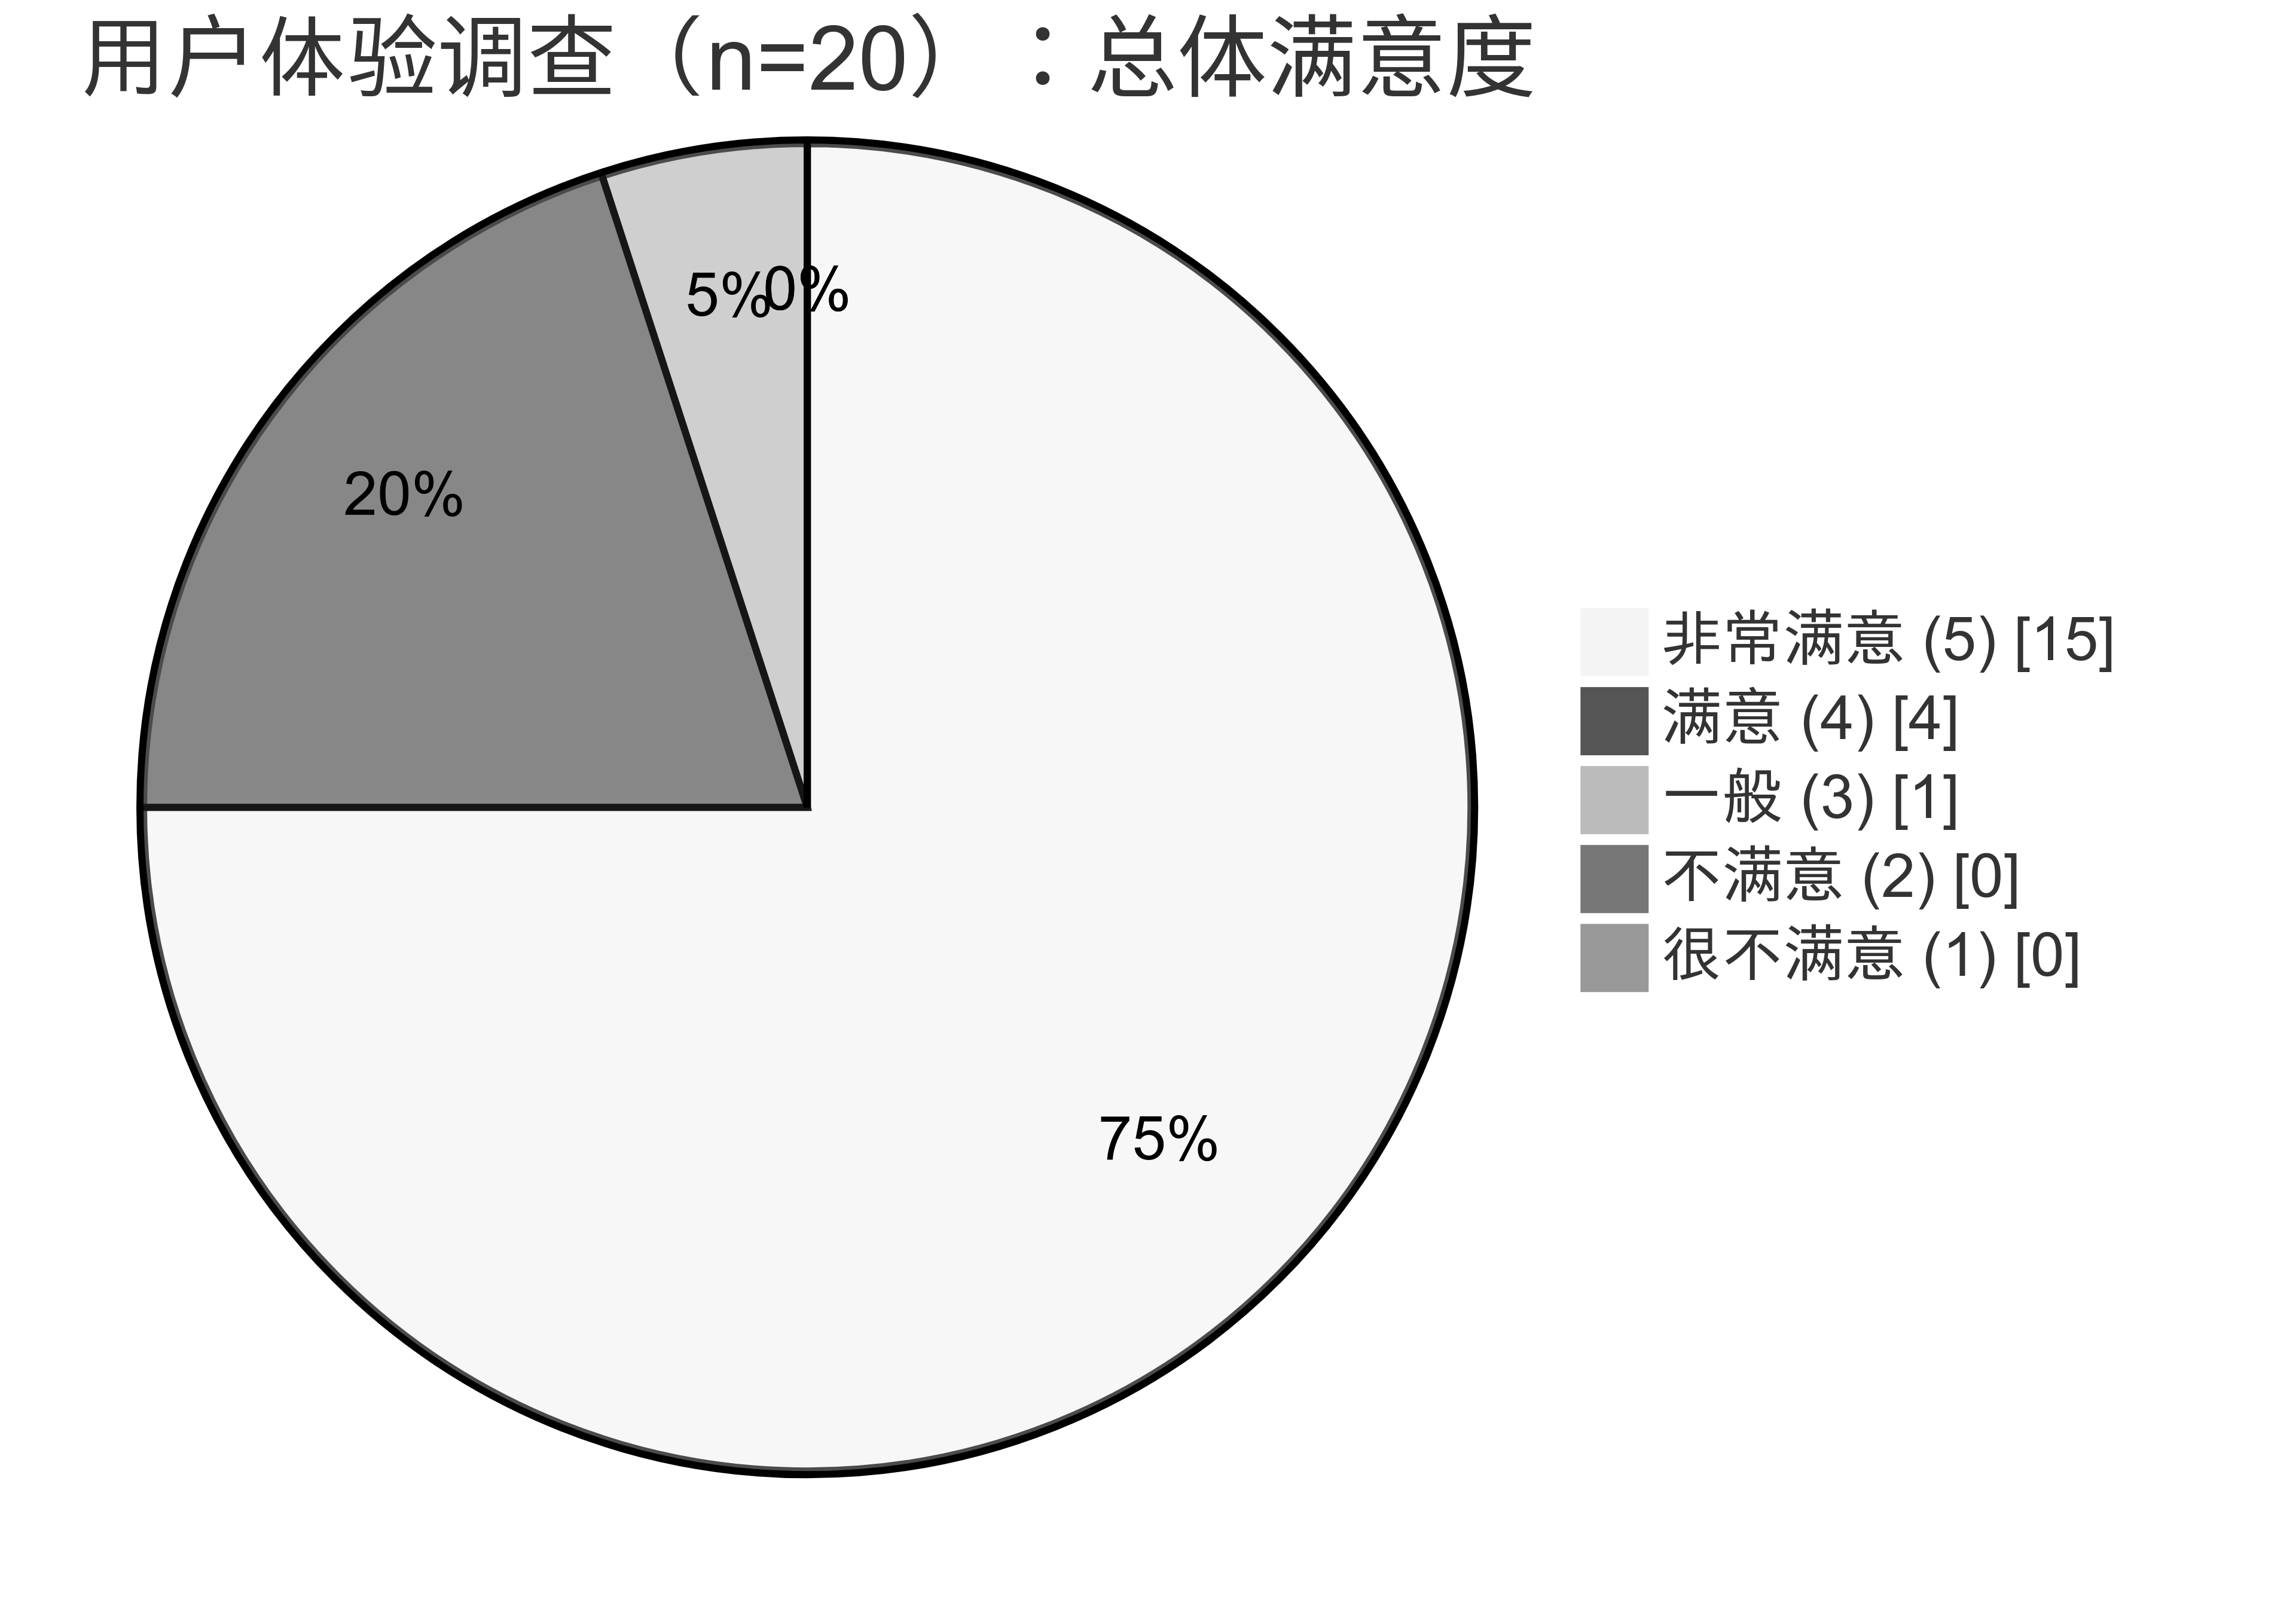
\includegraphics[width=0.8\textwidth]{chapters/fig-0/survey-satisfaction.png}
  \caption{用户问卷总体满意度分布(Likert 1--5,n=20)}
  \label{fig:survey-satisfaction}
\end{figure}
综合来看,用户体验评估表明本系统既能满足学术研究的易用性需求,也能在战术应用场景中支撑大规模并发与跨链互操作,为后续扩展到 JREAP、TTNT 与 SIMPLE 环境提供了良好基础。
